\documentclass[30pt,landscape]{sciposter}

\usepackage{pstricks}
\usepackage[pdftex]{graphicx}
\usepackage{multirow,array}
\usepackage{amsmath,amsthm,amssymb}
\usepackage{algorithmic}
\usepackage{fancybox}
\usepackage{multicol}
\usepackage{natbib}

\definecolor{SectionCol}{rgb}{1.0,1.0,1.0}    %% section heading color
\definecolor{BoxCol}{rgb}{0.5,0.0,0.0}

\newtheorem*{theorem}{Theorem}
\newtheorem*{lemma}{Lemma}
\newtheorem*{definition}{Definition}
\newtheorem*{conjecture}{Conjecture}

\newcommand{\R}{\mathbb{R}}

\renewcommand{\P}{\mathcal{P}}
\newcommand{\U}{\mathcal{U}}
\newcommand{\X}{\mathcal{X}}
\newcommand{\indicator}[1]{\mathbf{1}\left[{#1}\right]}
\newcommand{\x}{\mathbf{x}}
\newcommand{\KL}[2]{D\left(#1 \middle\| #2 \right)}
\newcommand{\norm}[1]{\left\| #1 \right\|}
\newcommand{\ip}[2]{\left\langle #1, #2 \right\rangle}

\DeclareMathOperator*{\argmin}{argmin}
\DeclareMathOperator{\err}{err}
\DeclareMathOperator{\Exp}{\mathbf{E}}
\DeclareMathOperator{\VC}{VC}

\begin{document}

\renewcommand{\thefootnote}{\fnsymbol{footnote}}
\renewcommand{\footlogo}{Typeset by pdf\LaTeX}
\renewcommand{\algorithmicrequire}{\textbf{Input:}}

\title{The Information-Theoretic Value of Unlabeled Data \\ in Semi-Supervised Learning}
\author{Alexander Golovnev (Harvard) \qquad \qquad D\'avid P\'al (Expedia, New York) \qquad \qquad Bal\'azs Sz\"or\'enyi (Yahoo, New York)}

\date{June 13, 2019}

\leftlogo[1.2]{harvard-logo}
\rightlogo[1.2]{yahoo-logo}
\conference{Thirty-sixth International Conference on Machine Learning (ICML 2019), June 9--15, 2019, Long Beach, California, USA}

\maketitle

\setlength{\parindent}{0em}
\setlength{\columnsep}{4cm}
\begin{multicols}{3}

\section*{The Problem}

\begin{itemize}
\item Distribution $D$ over a domain $X$
\item Unknown target function $f$ from a known hypothesis class $H \subseteq \{0,1\}^X$.
\item Learner receives $S = ((x_1, f(x_1)), (x_2, f(x_2)), \dots, (x_m, f(x_m)))$.
\end{itemize}

\vspace{1cm}

\textbf{Does knowing $D$ help?}

\section*{Sample Complexity}

\begin{itemize}
\item Learning algorithm outputs a classifier $g=A(S)$.
\item Its error is
$$
\err_D(g) = \Pr_{x \sim D}[f(x)\neq g(x)]
$$
\item Sample complexity is the smallest $m = m(\epsilon,\delta,D)$ such that for any target $f \in H$,
with probability $\ge 1 - \delta$
$$
\err_D(g) \le \epsilon
$$
\end{itemize}

\section*{Known Results}

\begin{itemize}
\item Without knowing $D$ the sample complexity is
$$
O \left( \frac{\VC(H) + \log(1/\delta)}{\epsilon} \right)
$$
Modulo log factors this is achieved by any constistent algorithm, i.e. ERM.

\vspace{0.5cm}

\item With knowledge of $D$, the sample complexity is at most
$$
O\left(\frac{\log N_{D,\epsilon/2} + \log(1/\epsilon)}{\delta} \right)
$$
where $N_{D,\epsilon/2}$ is $\frac{\epsilon}{2}$-covering number
of $H$ under the metric
$$
d(f,g) = \Pr_{x \sim D}[f(x) \neq g(x)] \; .
$$

\vspace{0.5cm}

\item Covering number upper bound
$$
N_{D,\epsilon} \le \left( \frac{4e}{\epsilon} \right)^{\displaystyle \frac{VC(H)}{1 - 1/e}}
$$

\vspace{0.5cm}

\item There exists a distribution $D$ such that \textbf{even with knowledge of $D$},
any algorithm needs at least
$$
\Omega \left( \frac{\VC(H) + \log(1/\delta)}{\epsilon} \right)
$$
labeled examples.

\vspace{0.5cm}

\item There are distributions $D$ such that any constistent algorithm
has sample complexity only $O(\log(1/\delta)/\epsilon)$.
\end{itemize}

\columnbreak

\section*{Summary of Known Results}

Fix $\epsilon$ and $\delta$.

\vspace{1cm}

\begin{center}
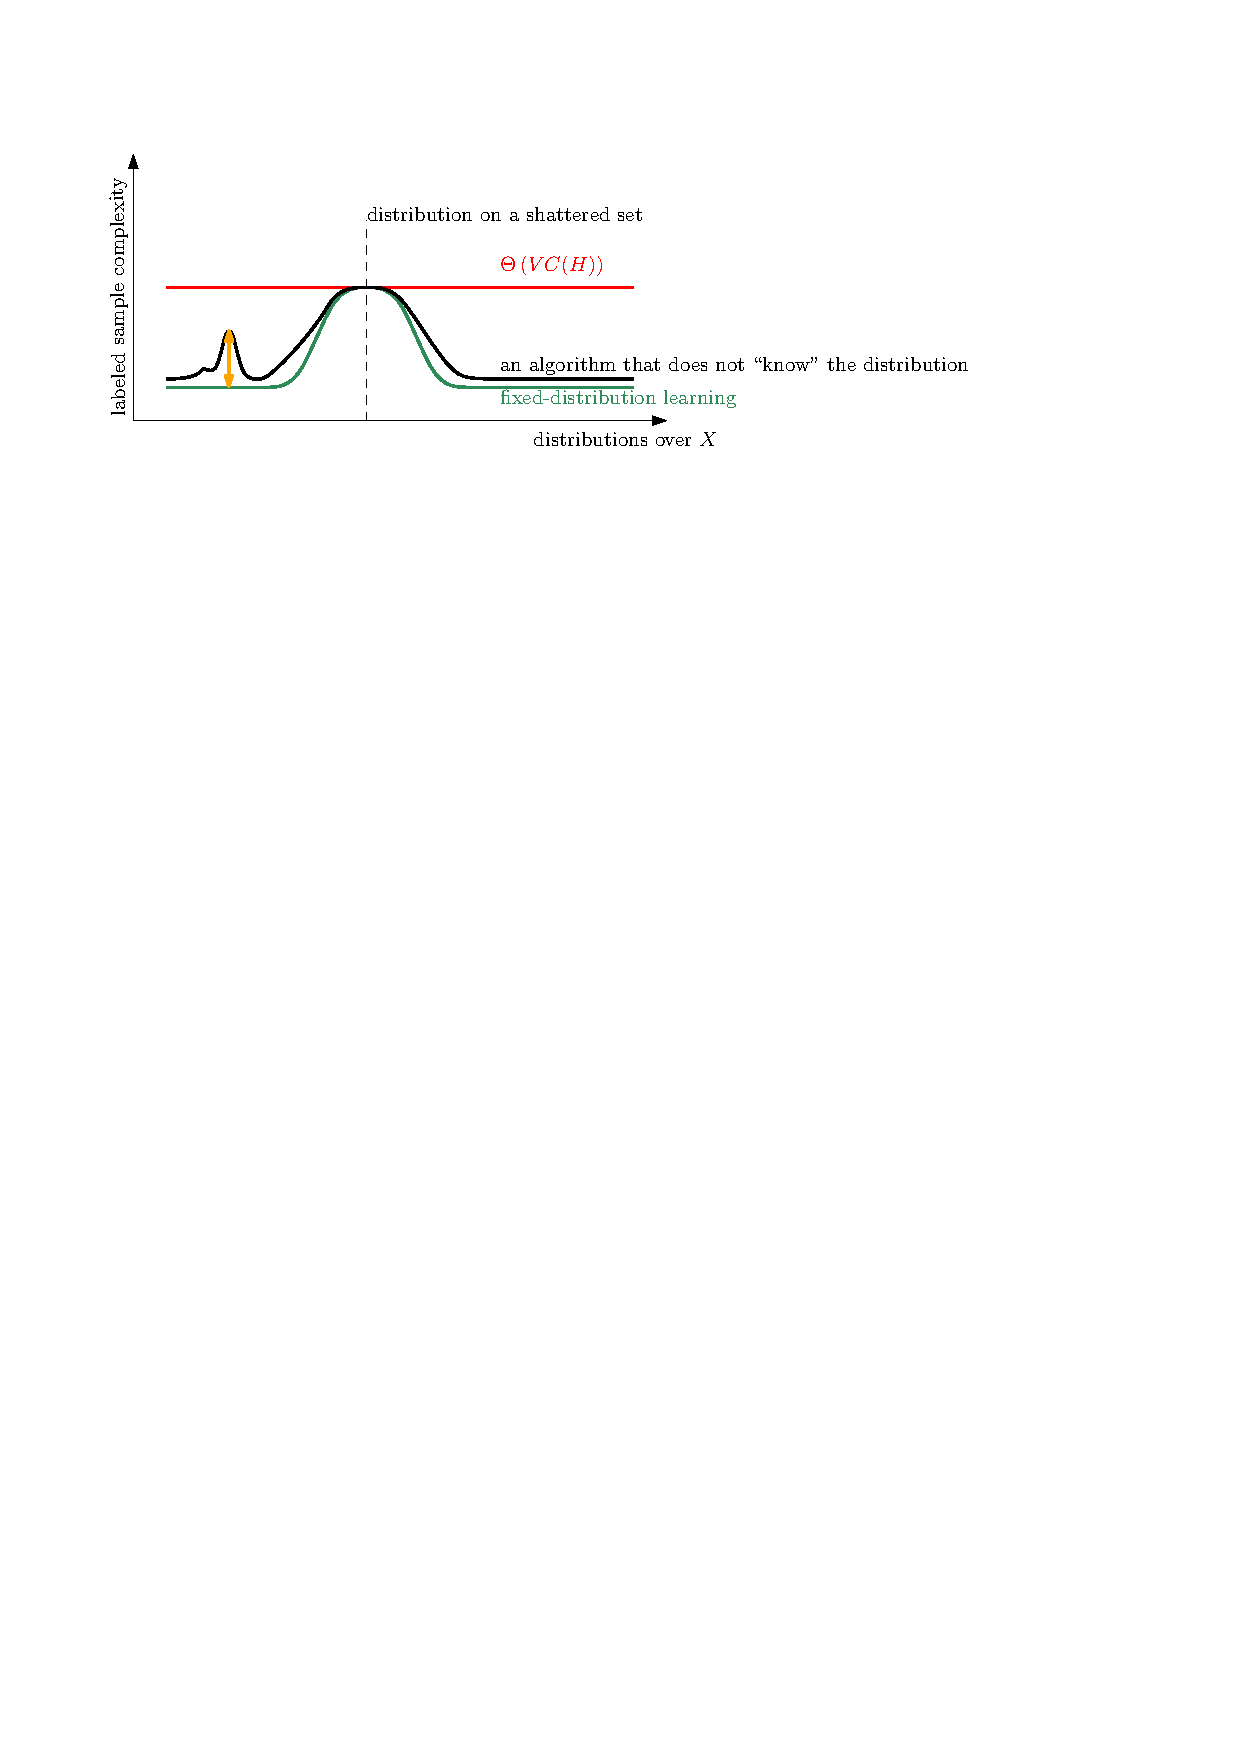
\includegraphics[width=0.3\textwidth]{figure-1}
\end{center}

\textbf{How big is the gap between the black and the green curve?}

\section*{Projections}

Domain is $X = \{0,1\}^n$ and hypothesis class is $H = \{h_1, h_2, \dots, h_n\}$
where
$$
h_i(x) = h(x[1], x[2], \dots, x[n]) = x[i]
$$
Vapnik-Chervonenkis dimension is $\VC(H) = \left \lfloor \log_2(n) \right \rfloor$.

\vspace{1cm}

\begin{theorem}
Fix $\epsilon$ and $\delta$. There are distributions $D_1, D_2, \dots, D_n$ such that
\begin{enumerate}
\item With knowledge of the distribution $D_i$, sample complexity is $O(1)$.
\item Without knowledge of $D_i$, sample complexity is $\Omega(\log n)$.
\end{enumerate}
\end{theorem}

\vspace{1cm}

\begin{center}
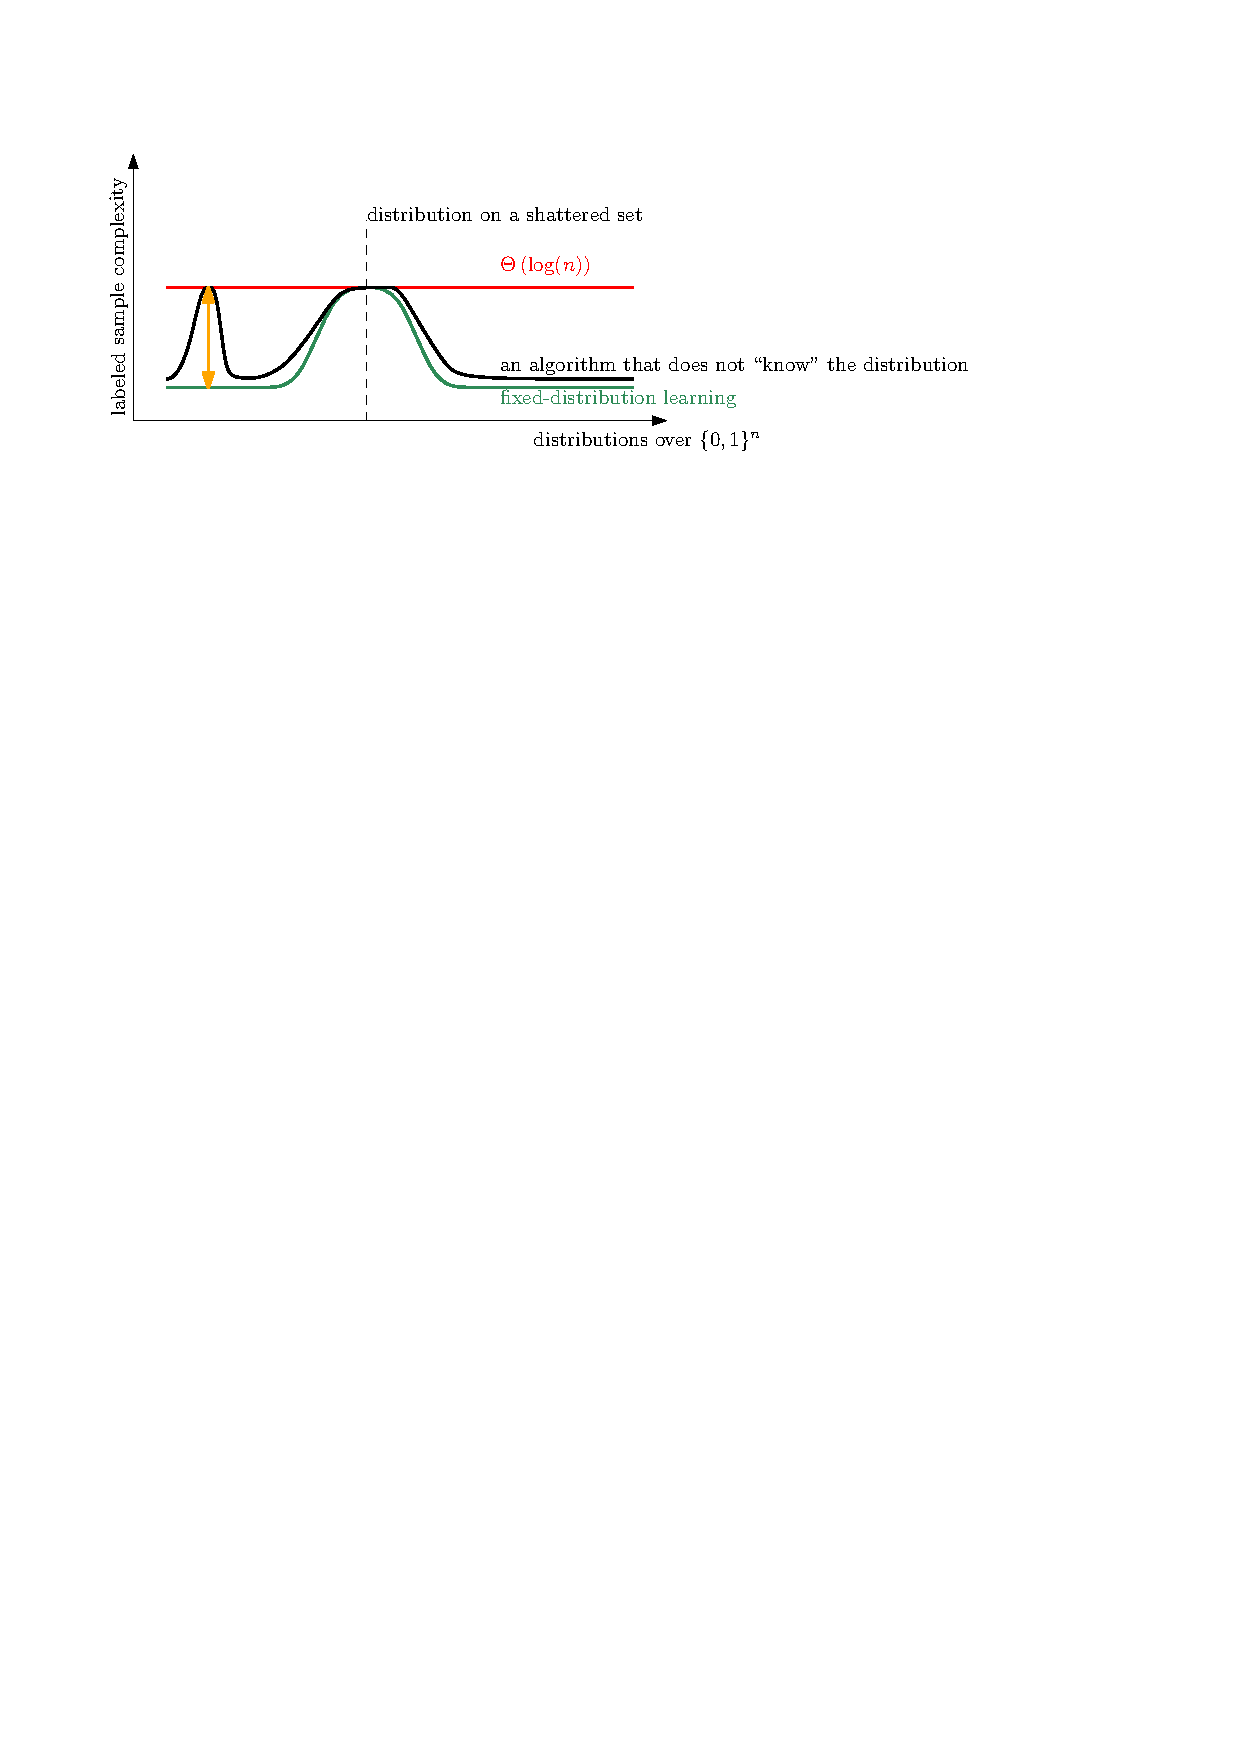
\includegraphics[width=0.3\textwidth]{figure-2}
\end{center}

\vspace{1cm}


Each $D_i$ is a product distribution such that
$$
\Pr_{x \sim D_i}[x[j] = 1] =
\begin{cases}
1/2 & \text{if $i = j$,} \\
\epsilon/4 & \text{if $i \neq j$.}
\end{cases}
$$

\columnbreak

\section*{Sketch of Proof}

\begin{itemize}
\item $D_i$ has $\epsilon/2$-cover of size $2$. Thus $O\left(\frac{\log N_{D,\epsilon/2} + \log(1/\delta)}{\epsilon} \right) = O(1)$
samples are enough to $\epsilon$-learn if $D_i$ is known to the learner.

\vspace{1cm}

\item Choose $i \in \{1,2,\dots,n\}$ at random.

\item Choose distribution $D_i$ and the target to be the projection $h_i$.

\item Algorithm that does \textbf{not} know $D_i$ and $h_i$, sees only the matrix
$$
\left(
\begin{array}{cccc|c}
x_{1}[1] & x_{1}[2] & \cdots & x_{1}[n] \  & \ y_1 \\
x_{2}[1] & x_{2}[2] & \cdots & x_{2}[n] \ & \ y_2 \\
\vdots & \vdots & \ddots & \vdots \ & \vdots \\
x_{m}[1] & x_{m}[2] & \cdots & x_{m}[n] \ & \ y_m \\
\end{array}
\right) \; .
$$

\item Column $x[i]$ matches column $y$.

\item If $m \le \log(n)$ then with constant probability at least one other column $x[j]$
matches column $y$.

\item Learner has to pick a column $i$ or $j$.
\end{itemize}

\vspace{1cm}

\textbf{For non-proper learners, the proof is more complicated.}

\section*{Conclusions}

\begin{itemize}
\item Unlabeled data help for projections.
\item For the class of \textbf{all functions}, unlabeled data do \textbf{not} help.
\item The problem is open for halfspaces and axis-aligned rectangles in $\R^n$,
and conjuctions and disjuctions in $\{0,1\}^n$. They have $\VC(H) = \Theta(n)$. \\
The gap could be potentially as big as $\Omega(n)$.
\end{itemize}

%%%%%%%%%%

\nocite{Benedek-Itai-1991,Ben-David-Lu-Pal-2008,Darnstadt-Simon-Szorenyi-2013,Hanneke-2016}
\bibliographystyle{plain}
\bibliography{biblio}


\end{multicols}

\end{document}
